\documentclass[a4paper,12pt]{article}

%%% Работа с русским языком
\usepackage{cmap}					% поиск в PDF
\usepackage{mathtext} 				% русские буквы в формулах
\usepackage[T2A]{fontenc}			% кодировка
\usepackage[utf8]{inputenc}			% кодировка исходного текста
\usepackage[english,russian]{babel}	% локализация и переносы

%%% Работа с картинками
\usepackage{graphicx}  % Для вставки рисунков
\graphicspath{{images/}{images2/}}  % папки с картинками
\setlength\fboxsep{3pt} % Отступ рамки \fbox{} от рисунка
\setlength\fboxrule{1pt} % Толщина линий рамки \fbox{}
\usepackage{wrapfig} % Обтекание рисунков текстом

%%% Работа с таблицами
\usepackage{array,tabularx,tabulary,booktabs} % Дополнительная работа с таблицами
\usepackage{longtable}  % Длинные таблицы
\usepackage{multirow} % Слияние строк в таблице

\begin{document}
	
\begin{center} 
	\hfill \break 
	\normalsize{ФЕДЕРАЛЬНОЕ ГОСУДАРСТВЕННОЕ АВТОНОМНОЕ }\\ 
	%\footnotesize{ФЕДЕРАЛЬНОЕ ГОСУДАРСТВЕННОЕ БЮДЖЕТНОЕ ОБРАЗОВАТЕЛЬНОЕ УЧРЕЖДЕНИЕ}\\ 
	%\footnotesize{ВЫСШЕГО ПРОФЕССИОНАЛЬНОГО ОБРАЗОВАНИЯ}\\ 
	\normalsize{ОБРАЗОВАТЕЛЬНОЕ УЧРЕЖДЕНИЕ ВЫСШЕГО ОБРАЗОВАНИЯ }\\ 
	\normalsize{НАЦИОНАЛЬНЫЙ ИССЛЕДОВАТЕЛЬСКИЙ УНИВЕРСИТЕТ}\\ 
	\normalsize{\textbf{«ВЫСШАЯ ШКОЛА ЭКОНОМИКИ»}}\\ 
	\hfill \break 
	\normalsize{\textbf{Московский институт электроники и математики\\ им. А.Н. Тихонова}}\\ 
	\hfill \break 
	\normalsize{Студенты учебной группы МСКМ 181:\\Чертенков В.И.\\Пехтерев Д.О.\\Горчавкина А.А.\\} 
	\hfill \break 
	\hfill \break 
	\hfill \break 
	\large{Техническая документация по проектной работе\\ \textbf{"Анализ отзывов о лекарственных препаратах в социальных медиа"}}\\ 
	\hfill \break 
	\hfill \break 
	%\normalsize{Аннатация по проектной работе %Междисциплинарная курсовая работа 
	%по направлению \\01.04.04 Прикладная математика\\ 
	\hfill \break 
	%студент образовательной программы магистратуры МСКМ 181\\ 
	\hfill \break 
	%Суперкомпьютерное моделирование в науке и инженерии}\\ 
	\hfill \break 
	\hfill \break 
\end{center} 
\hfill \break 
\begin{flushright} 
	%%\normalsize{Студент Курманов И.А.}\\ 
	\hfill \break 
	\hfill \break 
	\normalsize{Руководитель проекта \\ 
		\hfill \break 
		\normalsize{Артамонов С.Ю.} 
	\end{flushright} 
	\hfill \break 
	\begin{center} Москва 2019 \end{center} 
	\thispagestyle{empty} 
	
\section{Визуализация}
\subsection{Платформа Tableau Public}
При решении задачи анализа большого количества данных целесообразно применять удобные средства визуализации. В рамках нашего проекта было решено использовать платформу Tableau Public (public.tableau.com) – бесплатный редактор инфографики, позволяющий представить большинство типов данных в доступной форме. Это современное удобное средство построения разного рода зависимостей с возможностью последующей публикации на веб-ресурсах. Этот сервис позволяет работать с разными форматами данных - Microsoft Exel, Text, JSON, pdf и др. Полученные в результате рисунки автоматички сохраняютя в личном кабинете пользователя, что обеспечивает доступ к ним из любых устройств. Общий объем файлов пользователя ограничивается 10 Гб. Свое изображение можно дополнять текстом, а также прикреплять к нему гиперссылки и другие рисунки (см. рис. \ref{fig:fig1}).

\begin{figure}[h]
	\centering
	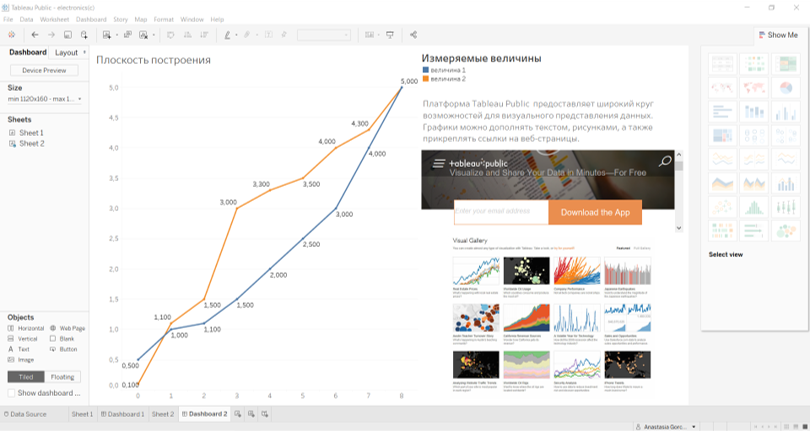
\includegraphics[width=1\linewidth]{fig1}
	\caption{Типичный вид интерфейса плтформы Tableau Public}
	\label{fig:fig1}
\end{figure} 

Соотношение занимаемой площади элементов и их порядок задается пользователем.	Результат работы можно публиковать на веб-страницах. При этом пользователь может интерактивно взаимодействовать с полотном: выделять зависимости, приближать изображение, изменять интервалы фильтрации.

\begin{figure}[h]
	\centering
	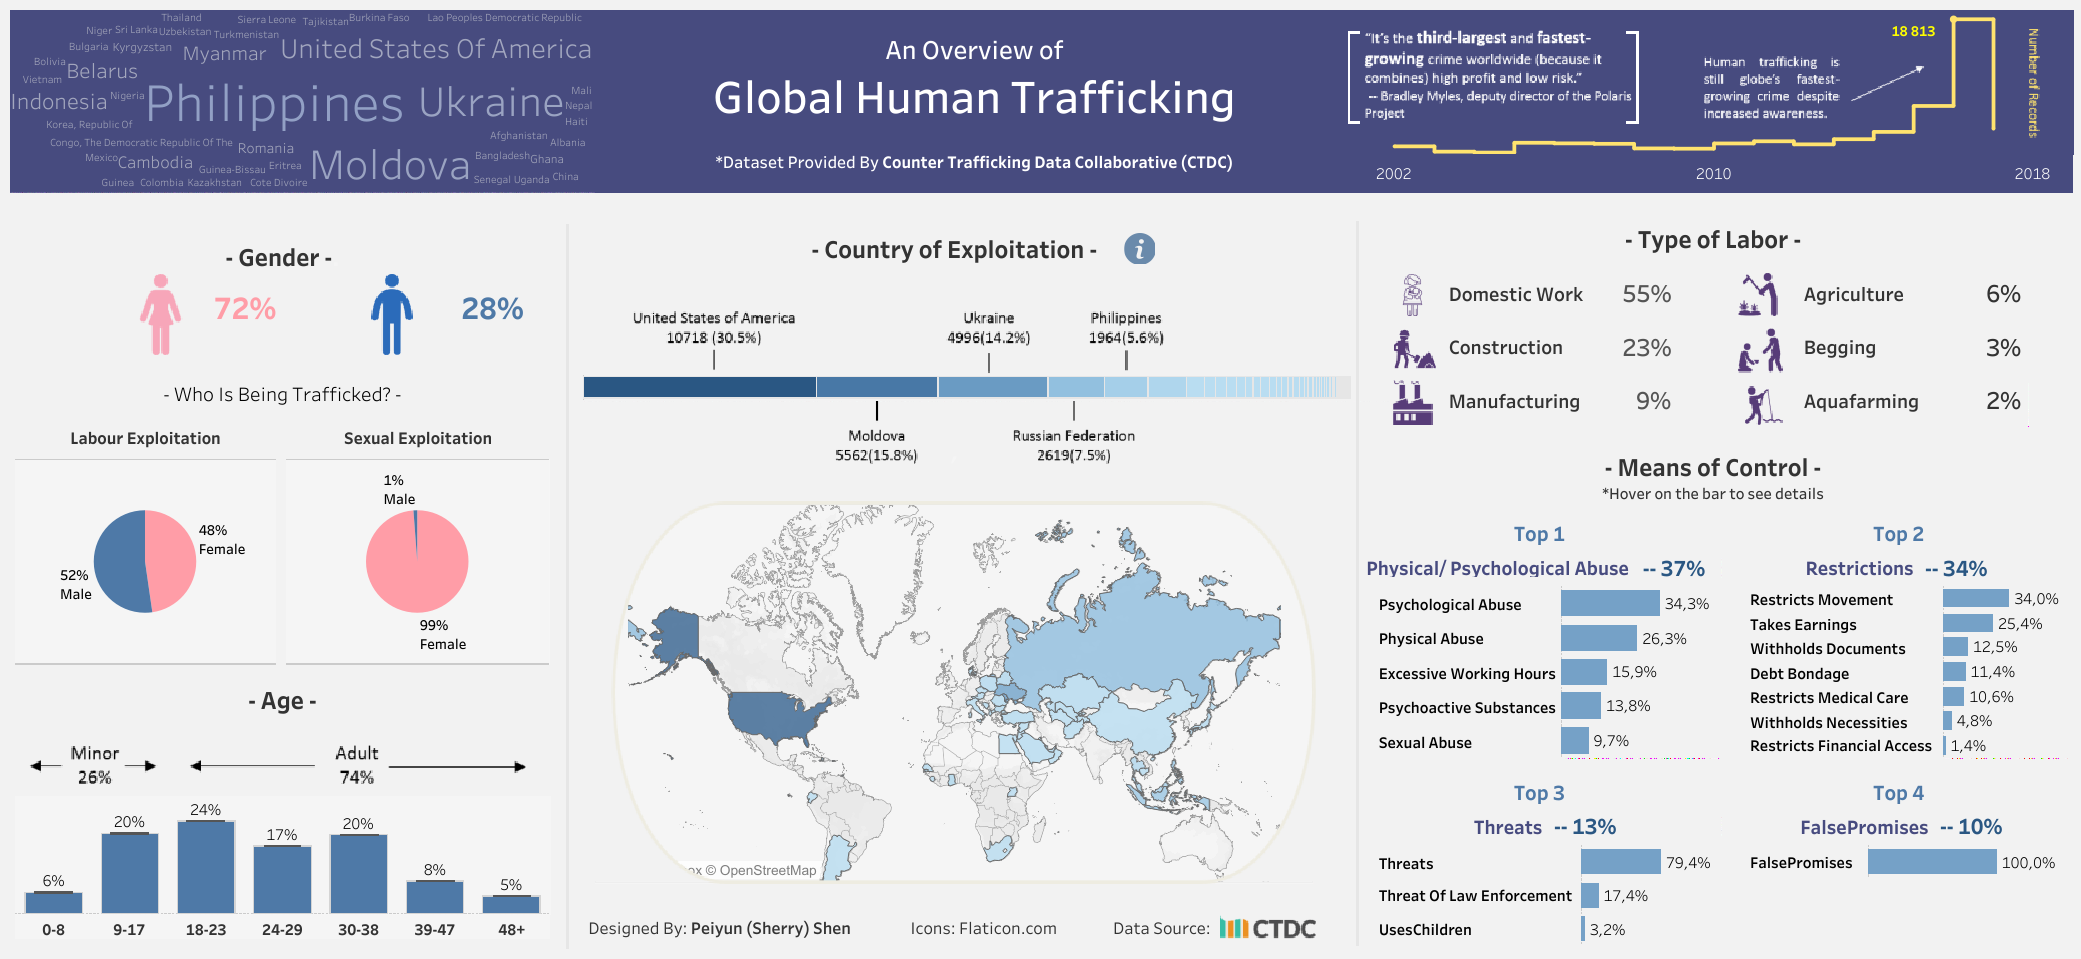
\includegraphics[width=1\linewidth]{fig2}
	\caption{Пример инфографики, выполненной в Tableau Public}
	\label{fig:fig2}
\end{figure} 

Приобтаемые навыки работы с платформой при построении графиков ROC-кривых алгоритмов классификации, подбора параметра C и различных вспомогательных изображений будут применяться в визуализации результатов анализа нашего конечного продукта.

\subsection{Облака слов}
Если алгоритм машинного обучения обрабатывает текстовые данные, полезно иметь представление о них. В частности, для алгоритма логистической регрессии мы строим облака слов \cite{tcloud} – изображение некоторого множества слов в соответствии с их критерием значимости. Критерий значимости определяется алгоритмом машинного обучения и представляет собой дествительное положительное или отрицательное число. 

Построение облака слов в Tableau Public выполнено на примере классификации методом логичтической регрессии. Для каждой категории данных получено изображение, где значимость слова определяется его близостью к центру, размером и интенсивностью оттенка. На рис. приведдены несколько из них для сравнения. В первой паре совпадений крайне мало, хотя обе категории тесно связаны с общим понятием «досуг». Во второй паре совпадений намного больше, хотя категории и кажутся и более отдаленными. Из этого можно сделать вывод, что нельзя выделить какое-то единственное множество слов разумного объема, используемое при описании чего-либо.

\begin{figure}[t]
	\centering
	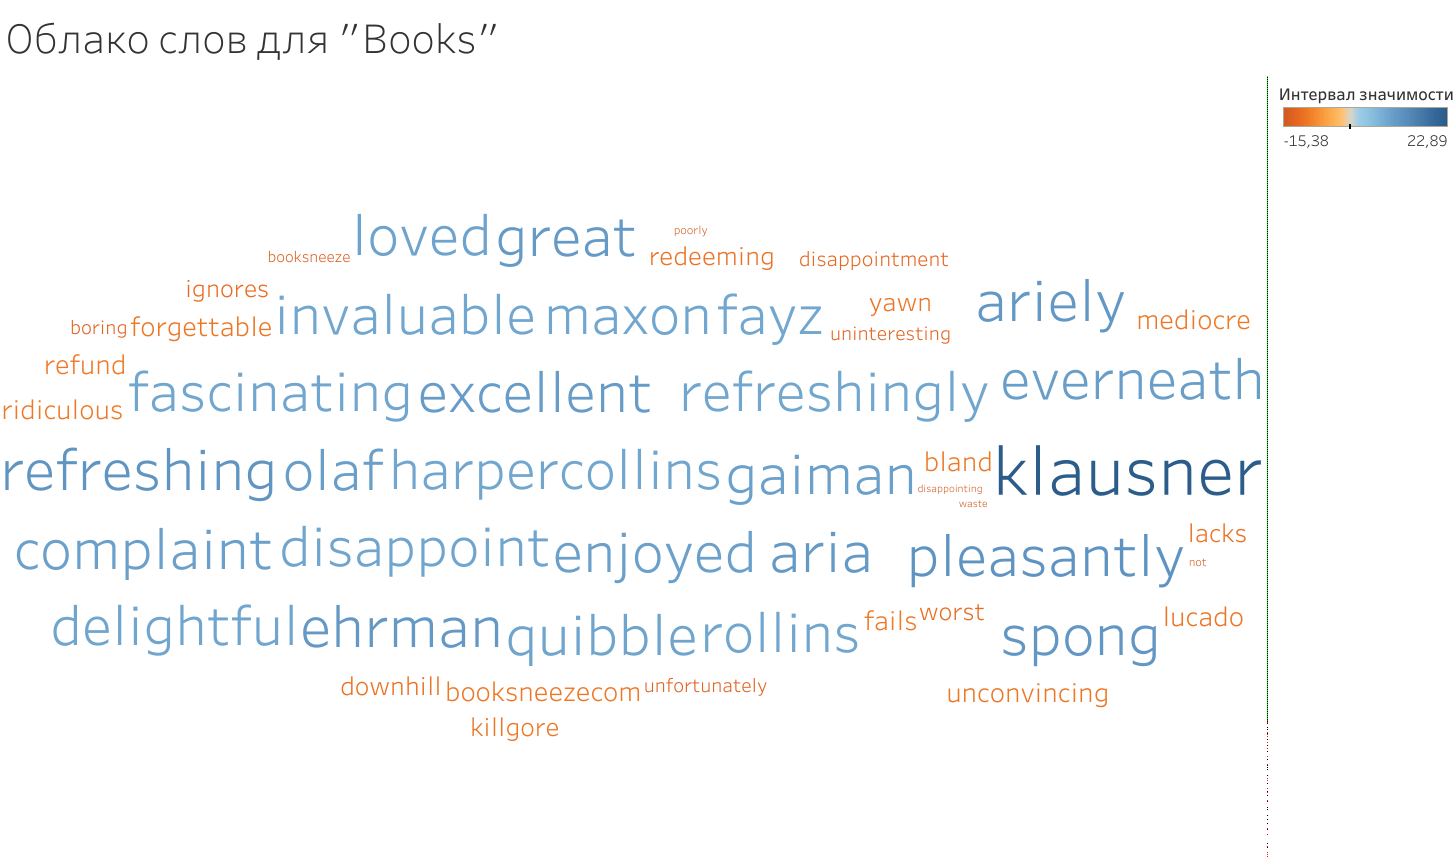
\includegraphics[width=0.45\linewidth]{1}
	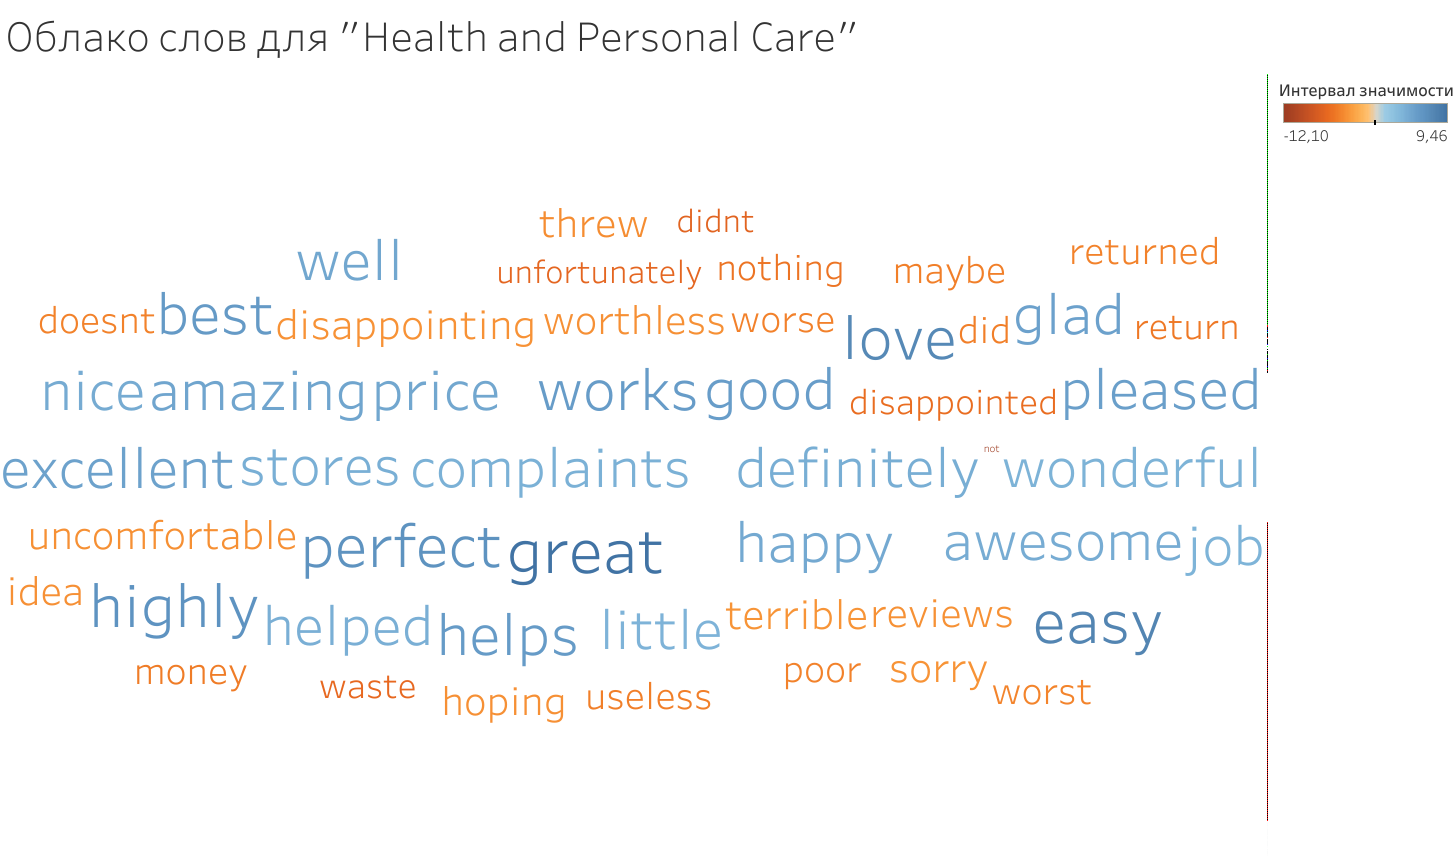
\includegraphics[width=0.45\linewidth]{2}
	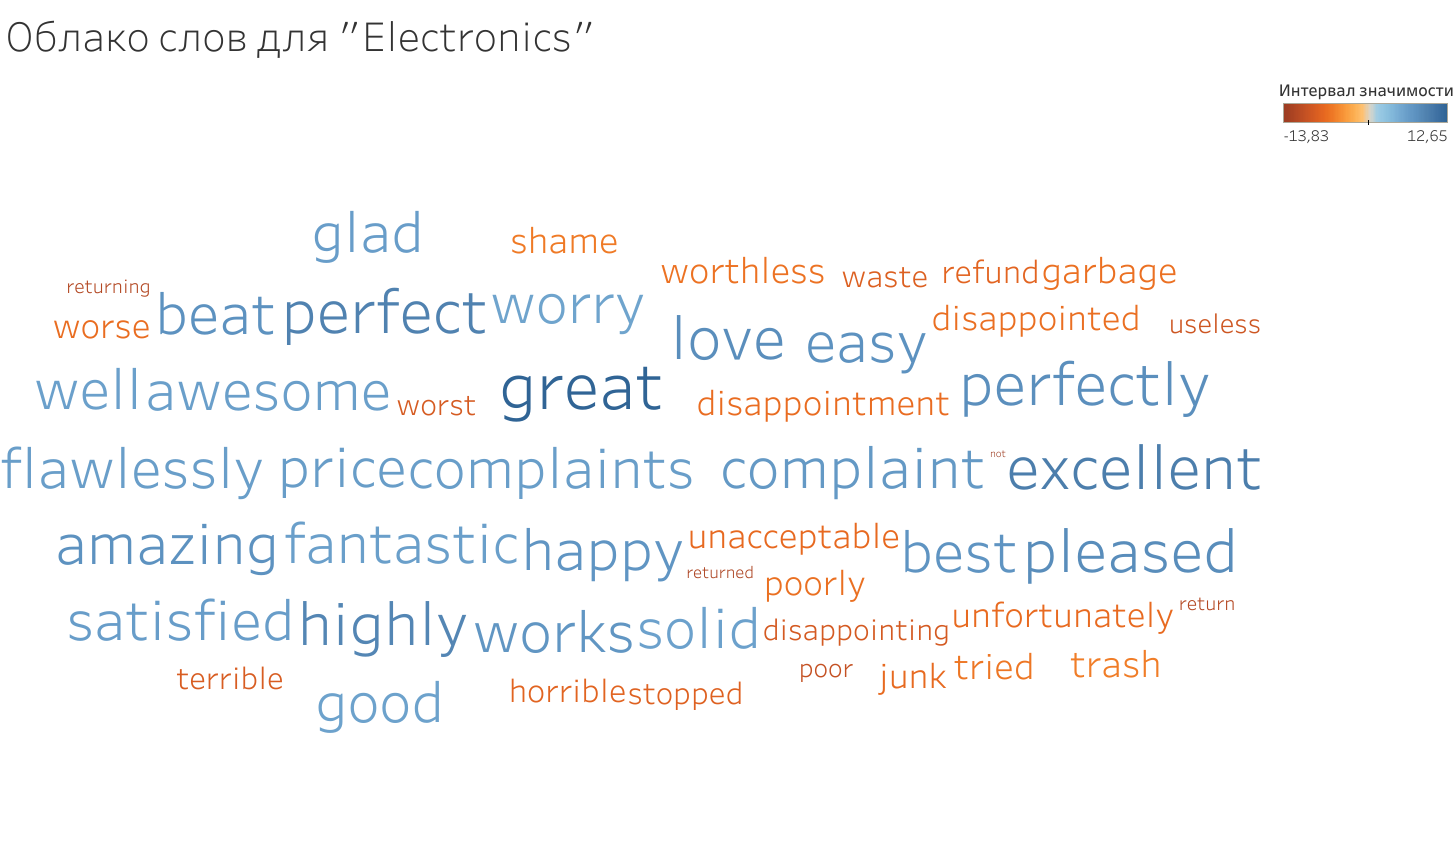
\includegraphics[width=0.45\linewidth]{3}
	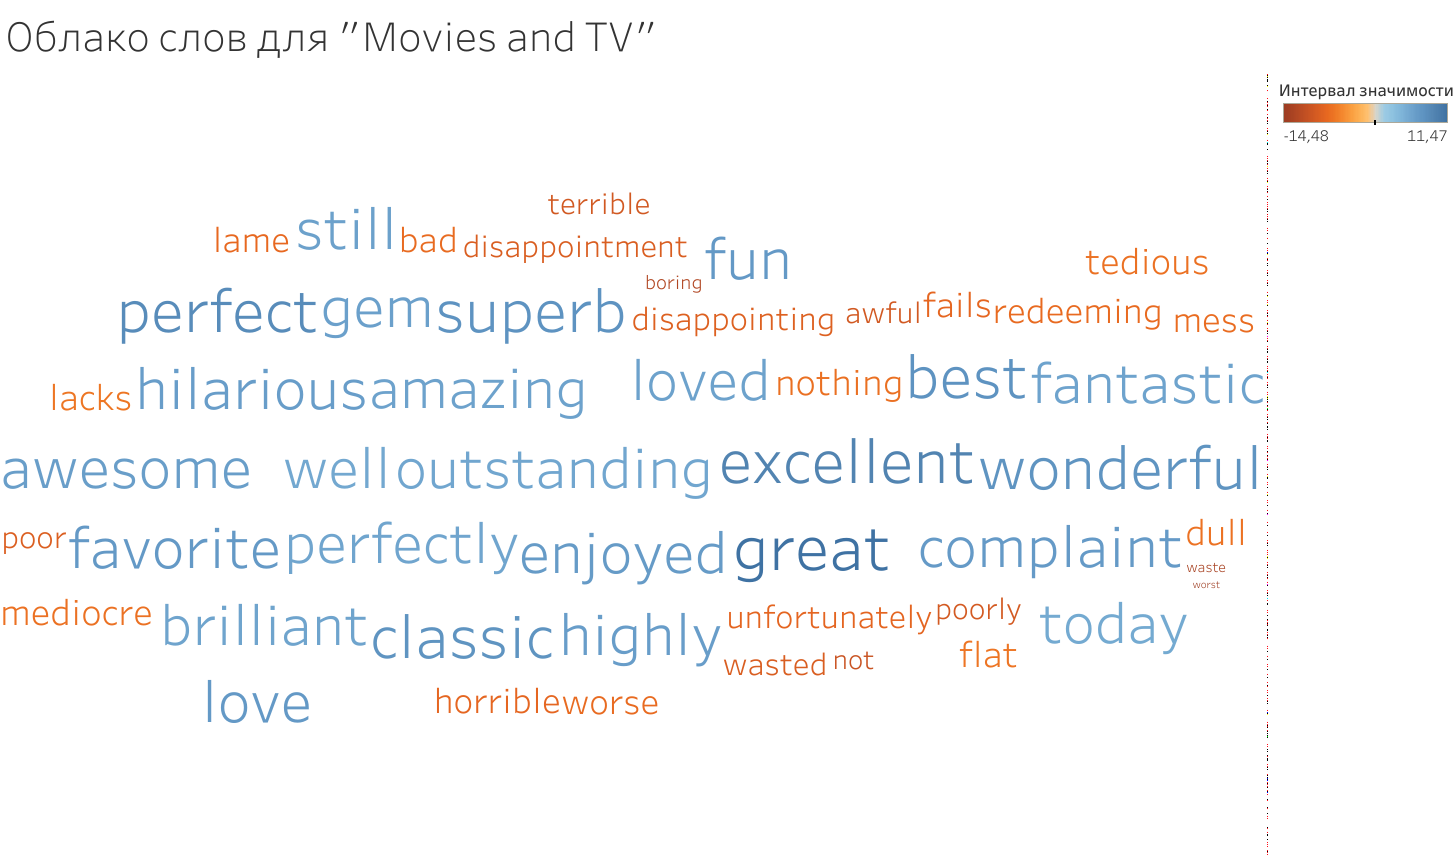
\includegraphics[width=0.45\linewidth]{4}
	\caption{Визуализация облака слов для разных категорий}
	\label{fig:tcloud1}
\end{figure}

\subsection{Визуализация процесса обучения}
На основе данных, полученных из метода логистическоой регрессии были построены кривые, визуализирующие процесс обучения. На рис. \ref{fig:c} видно, как зависит точность классификатора от параметра алгоритма С. Максимальная точность достигается в интервале от 1 до 10. 

\begin{figure}[h]
	\centering
	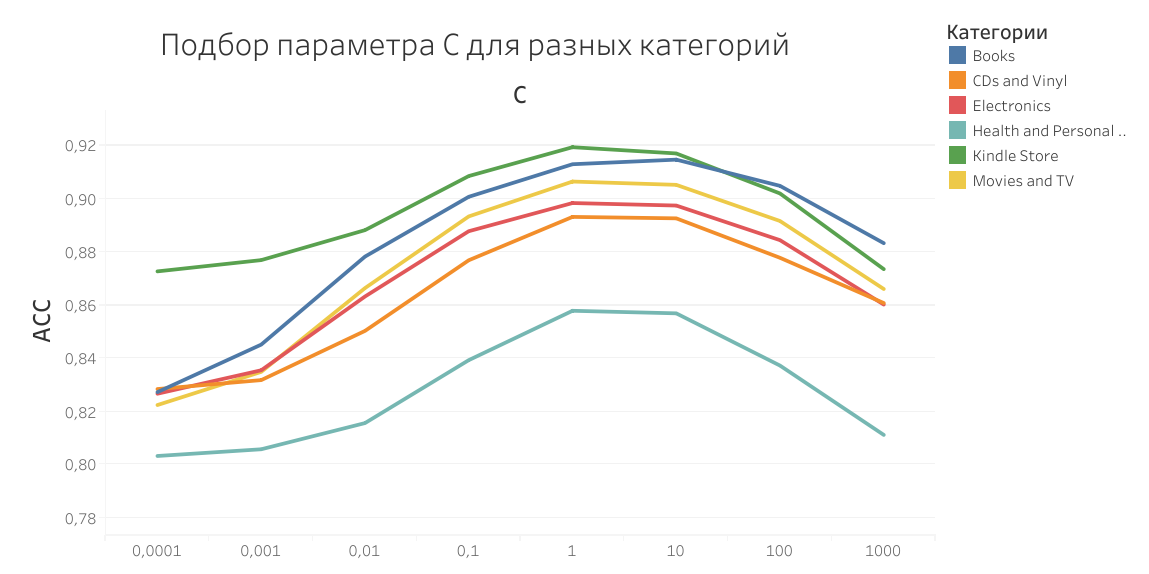
\includegraphics[width=0.9\linewidth]{c}
 
	\label{fig:c}
\end{figure} 
Для визуального представления точности работы классификатора удобно использовать ROC-кривые. На рис.\ref{fig:roc} такая кривая для категории Health and Personal Care. 

\begin{figure}[h]
	\centering
	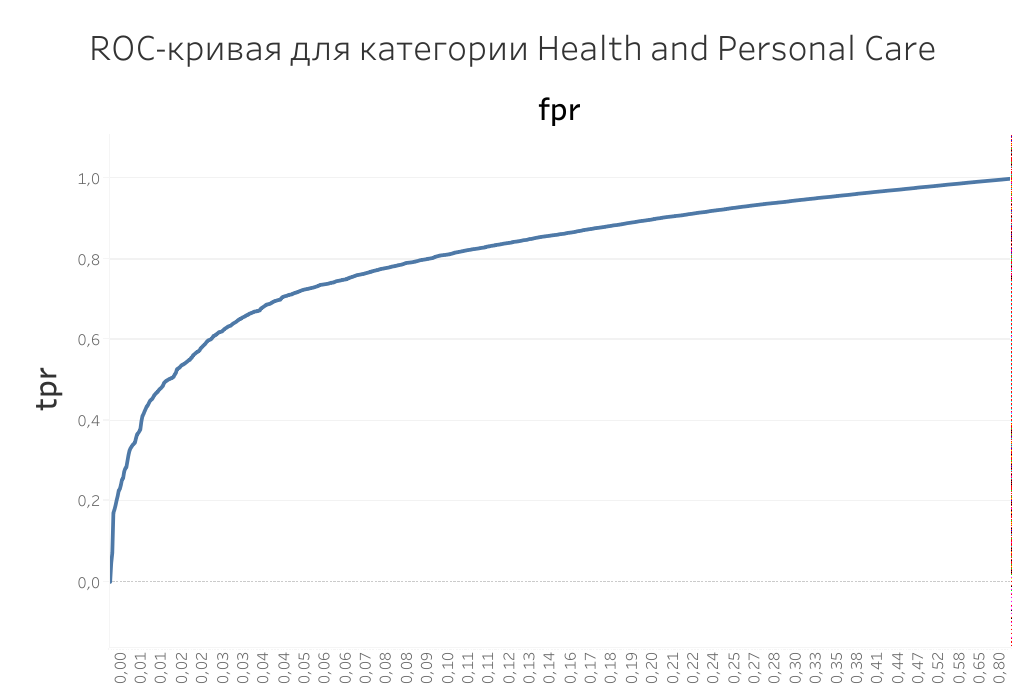
\includegraphics[width=0.9\linewidth]{roc}
 
	\label{fig:roc}
\end{figure} 
Конечно, приведенные зависимости можно построить и пользуясь другими ресурсами, но эта работа была проделана для определения особенностей платформы редактора. На данный момент мы знаем какую структуру должны иметь данные, их объемные ограничения, а также опробовали способы построение наиболее популярных форм визуализации. Полученный опыт будет применен для оформления конечного результата нашего продукта. 

\begin{thebibliography}{9}
	\bibitem{tcloud} Kaser O., Lemire D. Tag-cloud drawing: Algorithms for cloud visualization //arXiv preprint cs/0703109. – 2007.
\end{thebibliography}
\end{document}